\documentclass{article}
\usepackage[utf8]{vietnam}
\usepackage{graphicx}

\title{AI-1}
\author{Khac Minh}
\date{July 2019}

\begin{document}

\maketitle
% \selectlanguage{vietnam}

\section{Introduction}
    - Thứ 3 thầy Hưng giới thiệu về mô hình chung của Machine learning. 
    \begin{figure}[ht]
        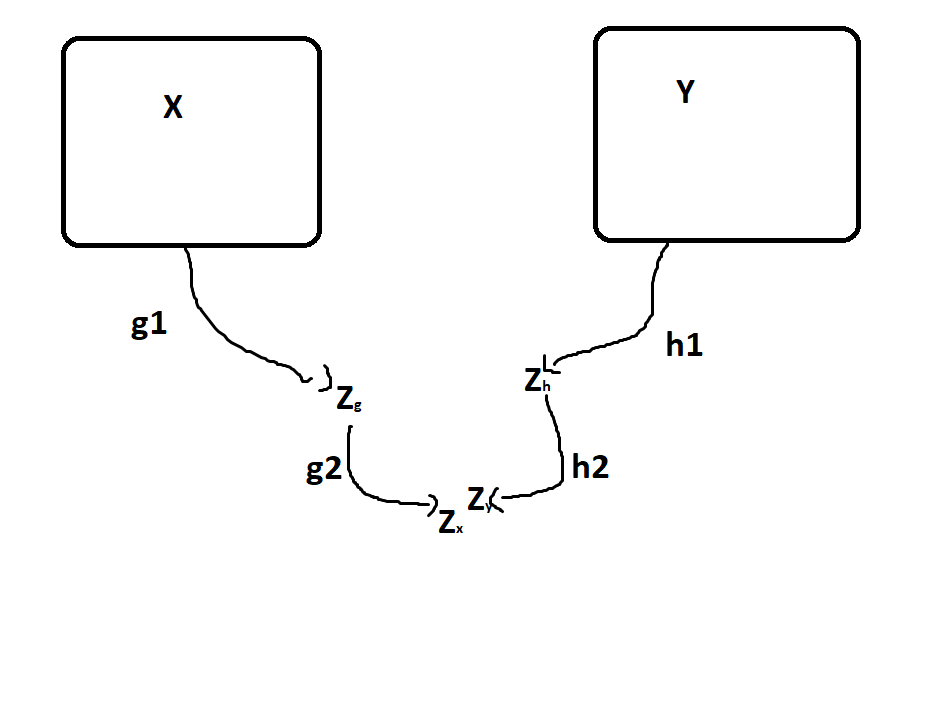
\includegraphics[width=10cm]{soDoKhoi.png}
        \caption{mô hình chung}
        \label{fig:figure2}
    \end{figure}
    -X là input, trong ví dụ PCA hôm thứ ba thì nó là tập ảnh gốc.
        + Trong ví dụ về định giá căn nhà thì nó là thông tin của các căn nhà.
        
    -g1 là hàm biến các input thành 1 vector dựa trên các vectơ cơ bản (Basis vector)
        Basis vector là các component, các đặc điểm nhận dạng của input. Vector Zg là hàm đặc trưng.
        
    - Nếu cần, g2 là hàm giúp biến vector Zg thành dạng mà có thể so sánh được. 
    
    - Trong bài PCA, PCA biến input(ảnh mặt người) thành vector và sau đó dùng coordinate đó reconstruct lại mặt người. 
    
    - Trong code của PCA, python tính ra được basis vector dùng PCA, tìm được ma trận tọa độ rồi nhờ đó tạo ra ảnh mới. 
    
    - Thầy Hưng cũng dạy cách so sánh dữ liệu luôn. Có 2 kiểu:
        + Lấy căn tổng bình phương độ khác nhau của từng coordinate của 2 ảnh chia cho kích cỡ ảnh.
        + Lấy căn tổng tích vô hướng của các coordinate. 
    
    - Thứ 4 thầy Hưng dạy về Linear Regression. 
    
    - Trong code của linear regression, python tính ra vector dựa vào thông tinh nhà xong ra được giá tiền.
    
    - Trong code của linear classification, nhờ vào các component, có thể ra được xác xuất sẽ là người là bao nhiêu phần trăm, ra hoa quả là bao nhiêu phần trăm.
\end{document}
